\chapter{Conditional Simulation Diagnostics of Frozen Forecasts}
\label{ch:calibration}
\section{Conditional diagnostics: useful discrimination without overall adequacy}

\subsection{Frozen target and diagnostic reference}

The completed conditional check targets original frozen OC alone. For each of its three origins, 999 complete branching-future paths were generated conditional on that origin's fixed fitted state, nuisance choices and original prehistory. Descendants can generate further descendants. All 2,997 paths completed; failed and unknown counts are zero. They are dependent-event paths under the model, not 2,997 independent earthquake samples. The observed-path exposure is a realised predictable compensator; it is not a Poisson future-count mean.

Each origin has 84 recorded coordinates, covering count, time gaps and dependence, spatial transforms and allocation, scores and subblocks. The 252 entries are not 252 independent diagnostic tests: immigrant exposure is a deterministic bookkeeping coordinate at each fixed origin, and total-exposure and trigger-exposure ranks coincide because their difference is that fixed constant. Those entries are retained for accounting, explicitly flagged in Appendix~\ref{app:audit12}, and add no independent evidence of adequacy. The spatial transforms draw on the probability-integral-transform tradition \citep{Rosenblatt1952,Schoenberg2003}. A coordinate's insertion interval is

\begin{equation}
\left[\frac{1+\#\{S^{(r)}<S^{\rm obs}\}}{1000},\quad
\frac{1+\#\{S^{(r)}\leq S^{\rm obs}\}}{1000}\right].
\end{equation}

The resolution is 0.001. Boundary ranks are finite reference comparisons, not zero probability or exact population tail probabilities. Ties can create wide intervals. This descriptive collection has no asserted omnibus significance test, and its coordinates are not separate unadjusted discoveries. Empirical reference intervals describe simulated catalogues, not confidence intervals for fitted parameters or scientific validity.

\subsection{Discrepant and ordinary-looking results coexist}

\begingroup\footnotesize\setlength{\tabcolsep}{2pt}\renewcommand{\arraystretch}{1.18}
\begin{longtable}{@{}>{\raggedright\arraybackslash}p{0.1800\textwidth}>{\raggedright\arraybackslash}p{0.1800\textwidth}>{\raggedright\arraybackslash}p{0.1800\textwidth}>{\raggedright\arraybackslash}p{0.1800\textwidth}>{\raggedright\arraybackslash}p{0.1800\textwidth}@{}}
\toprule
{}Origin & Recorded count & Supplied simulated count interval & Count insertion interval & Selected diagnostic evidence \\
\midrule\endfirsthead
\toprule
Origin & Recorded count & Supplied simulated count interval & Count insertion interval & Selected diagnostic evidence \\
\midrule\endhead
\midrule\multicolumn{5}{r}{\emph{Continued on next page}}\\
\endfoot
\bottomrule\endlastfoot
{}Early & 79 & 121-453 & [0.001, 0.001] & Gap KS, serial statistic and spatial KS exceed every reference \\
{}Middle & 167 & 90-398 & [0.704, 0.712] & Ordinary total hides yearly concentration and dependence \\
{}Late & 69 & 69-279 & [0.021, 0.028] & Marginal gap/spatial KS ordinary; dependence and variance discrepant \\
\end{longtable}\endgroup

Early count is below all 999 simulated counts. Its exposure and trigger exposure are also below all references. Its gap KS is 0.222245 and spatial Rosenblatt KS is 0.167335, each above every reference. Yet the time event-logsum insertion is 0.583, the censored terminal tail 0.111 and within-cell absolute maximum 0.187. The model does not fail every coordinate in the same way.

Middle total count looks ordinary, but the five yearly counts are 12, 4, 8, 116 and 27. Its subblock balance maximum has insertion 0.998; the gap serial statistic exceeds all references. Its conditional-location score insertion is 0.364 and within-cell density score 0.312, while spatial KS, cross dependence and allocation show discrepancies. A satisfactory-looking total or score coordinate does not settle concentration or dependence.

Late gap KS has insertion 0.676 and spatial KS 0.810, yet serial dependence has insertion 0.998, the spatial cross statistic 0.992, and dimensionless location variance exceeds every reference. Across origins, cell 4 observed counts 15, 7 and 8 are below conditional allocations 23.493717, 16.132286 and 14.770085. These allocations sum conditional probabilities at observed event times; they are not unconditional event-count means. Empty-cell ties require particular care: one zero count has insertion [0.001, 0.563], which cannot be summarized by its lower endpoint.

Raw score totals also depend on target count and density measure. Early total location and joint scores exceed all simulated totals while its count is below all simulated counts; this does not validate its probabilities. Immigrant exposure ties identically across paths within a fixed state by construction. Neither that deterministic tie nor count-dependent mark totals validates the underlying recipe.

\subsection{Diagnostic scope}

OC shows material conditional diagnostic discrepancies in all three origins: early count and several dependence/spatial coordinates, middle concentration and dependence, and late dependence and location variance. The fixed-state forecast therefore lacks demonstrated conditional adequacy. That original coordinate-wise conclusion was descriptive rather than an omnibus rejection. EP was absent from that historical OC-only simulation experiment. The subsequent comparative conditional evaluation in Section~\ref{sec:s05-completed} includes EP and the declared within-origin omnibus statistics. Simulation-based forecast testing separates these questions \citep{Schorlemmer2007,Zechar2010}. Fitting, selection, measurement and catalogue-revision uncertainty are excluded by fixing the state. Later training histories include earlier target periods; separate per-origin simulations do not define a coherent cross-origin joint null. Cross-window patterns remain descriptive. Heavy-tailed productivity has infinite second moment under the fixed mark recipe, and normal/CLT count inference is not used. A censored terminal tail is survival information, not an additional completed gap.

The conditional diagnostic report and current evidence index retain the coordinate-level source and audit scope. All paths received identity/count/mark/exposure checks; independent full 84-coordinate raw replay covered nine paths, three prescribed indices per origin, not all 2,997 complete vectors. These are original audit outcomes. This edition recovered the simulation and diagnostic records and checked their hashes and source identities; it did not repeat that simulation or diagnostic campaign.



\section{Complete diagnostic record and subsequent evaluation}
Appendix~\ref{app:custody}, Section~\ref{app:audit12}, retains the complete coordinate tables and origin-specific rank figures, their reference definitions, and the independent numerical audit. The compact summary above and that full record describe the same frozen OC experiment.

The subsequent score-concentration and catalogue-robustness evaluation retained both discrepant and ordinary-looking diagnostics. Its completed results appear in Chapter~\ref{ch:external}; the frozen OC calibration target was not replaced by that follow-on.

\section{Completed conditional forecast calibration}

\label{sec:s05-completed}

Each model and California origin has 999 conditional simulated futures and its observed vector. The following tests condition on the fitted state and past history; they do not integrate parameter-estimation uncertainty.

\begin{table}[htbp]\centering\caption{Conditional count, original minimum-rank and continuous-coordinate pooled tests. All p-values use their declared inclusive-tail conventions.}\label{tab:s05-completed}

\begin{tabular}{llrrrr}\toprule Model & Fold & Conditional $N$ & Min-rank & Quadratic & Fisher-type\\\midrule

OC & 0 & 0.002 & 0.070 & 0.004 & 0.001 \\

OC & 1 & 0.594 & 0.075 & 0.003 & 0.004 \\

OC & 2 & 0.056 & 0.069 & 0.007 & 0.012 \\

EP & 0 & 0.002 & 0.070 & 0.004 & 0.002 \\

EP & 1 & 0.698 & 0.075 & 0.005 & 0.006 \\

EP & 2 & 0.036 & 0.069 & 0.009 & 0.008 \\

\bottomrule\end{tabular}\end{table}

The conditional count summary retains lower and upper inclusive empirical tails and reports twice the smaller tail, capped at one. The original minimum-rank test is retained with its exclusions and tie behaviour; it is not replaced by the continuous-coordinate statistics.

The pooled quadratic statistic uses eight declared coordinates: total exposure, time-event log sum, gap KS, gap serial correlation, spatial Rosenblatt KS maximum, absolute spatial cross-correlation, and dimensionless location-log-density mean and variance. Standardization and the ridge-regularized covariance are computed symmetrically on the observed vector plus all simulated vectors. The Fisher-type statistic is the preserved $-\sum_j\log\widetilde p_j$, not an independently calibrated chi-square reference or an assumption of independent coordinates. Both statistics use the inclusive upper rank in the same symmetric pool.

\begin{table}[htbp]\centering\caption{Retained-coordinate and tie diagnostics. Equal counts include the observed vector and every exactly tied pooled statistic.}

\begin{tabular}{llrrr}\toprule Model & Fold & Min-rank coordinates & Quadratic equal & Fisher equal\\\midrule

OC & 0 & 82 & 1 & 1 \\

OC & 1 & 82 & 1 & 1 \\

OC & 2 & 82 & 1 & 1 \\

EP & 0 & 82 & 1 & 1 \\

EP & 1 & 82 & 1 & 1 \\

EP & 2 & 82 & 1 & 1 \\

\bottomrule\end{tabular}\end{table}

Continuous does not automatically mean tie-free: coordinate duplicates and equality with the observed statistic are retained in the public aggregate and interpreted conservatively. This is the declared conditional calibration and pooled omnibus scope. No CSEP L-, M- or S-test results are inferred, and a non-rejection is not proof that the model or physical inhibition mechanism is correct. The independent reconstruction coverage is reported separately below; saved arithmetic checks and raw replay remain distinct forms of evidence.

\begin{figure}[htbp]\centering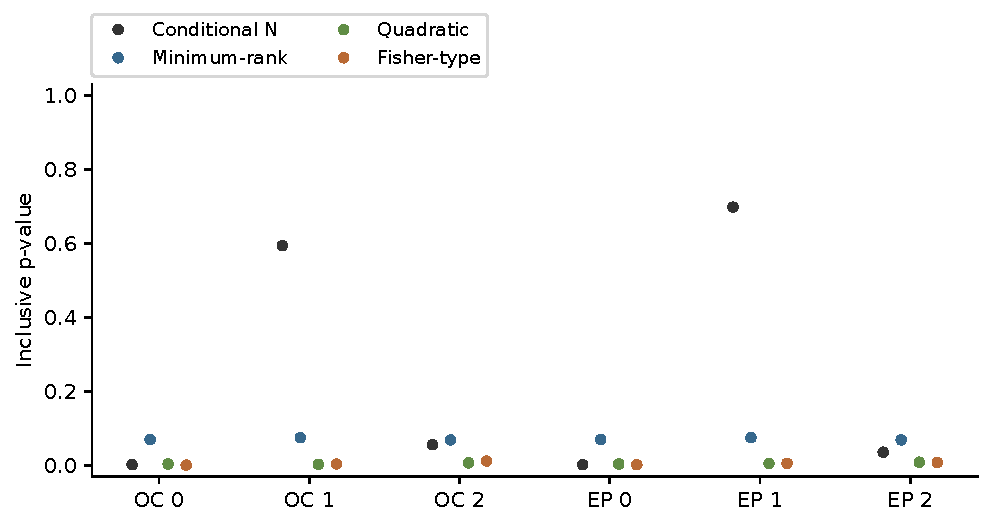
\includegraphics[width=\textwidth]{s05_conditional_pvalues.pdf}\caption{Reported inclusive conditional/pooled p-values.}\end{figure}

\begin{center}\begin{tabular}{llrrl}\toprule Model & Fold & Completed futures & Planned futures & Status\\\midrule

OC & 0 & 999 & 999 & resolved \\

OC & 1 & 999 & 999 & resolved \\

OC & 2 & 999 & 999 & resolved \\

EP & 0 & 999 & 999 & resolved \\

EP & 1 & 999 & 999 & resolved \\

EP & 2 & 999 & 999 & resolved \\

\bottomrule\end{tabular}\end{center}

Both continuous-statistic omnibus procedures reject at the declared five-percent level for each model and origin, while the retained minimum-rank procedure does not. Thus the EP score advantage is not a conditional-adequacy certificate. These are separate within-origin tests, not a joint cross-origin or model-selection-adjusted rejection. The historical OC full-vector audit remains separate.

% Additive replacement audit-scope text for 12_s05_completed.tex.
% Preserve every existing calibration p-value, table and figure.
The original completed independent closure reconstructed count, marks, immigrant and triggering exposure, temporal event logs, and spatial point, location and joint scores directly from all 5,994 saved OC and EP futures (999 per model and origin). It also reconstructed all 84 diagnostic coordinates and all 11 event-detail columns on EP indices 0, 249, 499, 749 and 998 in each of the three origins, giving 15 predeclared full-vector replays. Count identities are exact; finite numerical discrepancies satisfy the declared score, diagnostic and spatial-CDF tolerances. This extends the earlier nine-path native sample and zero-full-vector scope; it does not assert full spatial-PIT replay on all futures.

The independent reconstruction uses incomplete-beta line integrals and a separately implemented positive-polar rectangle-integration kernel. The scoring route and source identities are documented in \path{reproduction/regional/README.md}.

\begin{center}\begin{tabular}{lr}\toprule Independent closure quantity & Value\\\midrule
Independent raw point-score paths & 5994 \\
EP paths with all 84 diagnostics & 15 \\
Maximum point-score error (nats) & 1.17143e-09 \\
Maximum full-vector score error (nats) & 9.09495e-12 \\
Maximum other diagnostic error & 8.18545e-12 \\
Maximum spatial-CDF error & 6.66134e-15 \\
Maximum event-log error (nats) & 1.10134e-13 \\
Maximum gap error & 1.15463e-14 \\
\bottomrule\end{tabular}\end{center}


